\documentclass[11pt]{article}
\usepackage{geometry, graphicx, amssymb, amsmath, epstopdf}
\geometry{letterpaper}
\DeclareGraphicsRule{.tif}{png}{.png}{`convert #1 `dirname #1`/`basename #1 .tif`.png}
\newcounter{eoceSolCh}
\setcounter{eoceSolCh}{0}
\newcommand{\eoceSolCh}[1]{
\refstepcounter{eoceSolCh}\noindent\textbf{\arabic{eoceSolCh}\hspace{2mm}#1}

\addvspace{2mm}

}
\newcounter{eoceSol}[eoceSolCh]
\newcommand{\eoceSol}[1]{\refstepcounter{eoceSol}\noindent\small\textbf{\arabic{eoceSolCh}.\arabic{eoceSol}}\hspace{2mm}#1\addtocounter{eoceSol}{1}

\addvspace{1mm}

}
\begin{document}


%%%%%%%%%%%%%%%%%%%%%%%

\setcounter{eoceSolCh}{2}
\eoceSolCh{Distributions of random variables}

\eoceSol{Plots below. (a) 0.09. (b) 0.07. (c) 0.59. (d) 0.05.}
%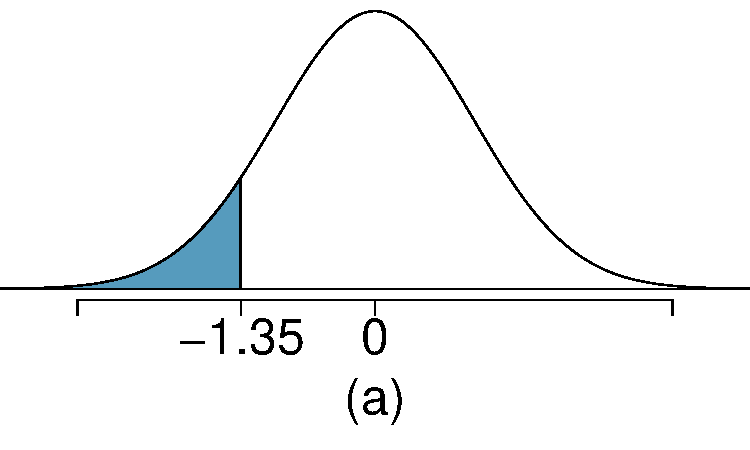
\includegraphics[width=0.2\textwidth]{03/figures/eoce/zltNeg}
%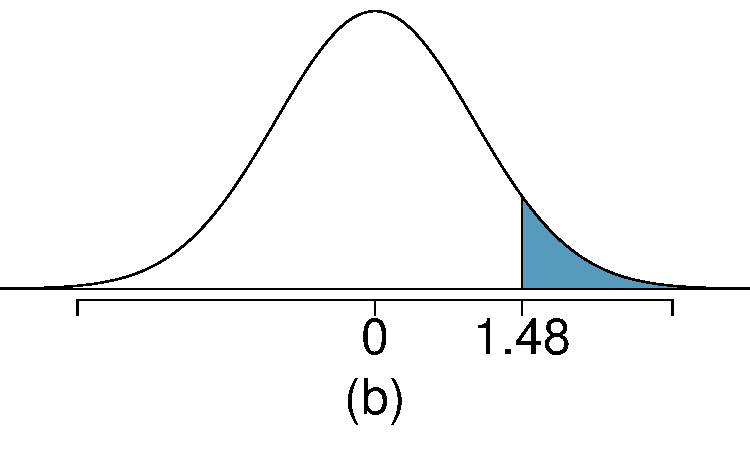
\includegraphics[width=0.2\textwidth]{03/figures/eoce/zgtPos}
%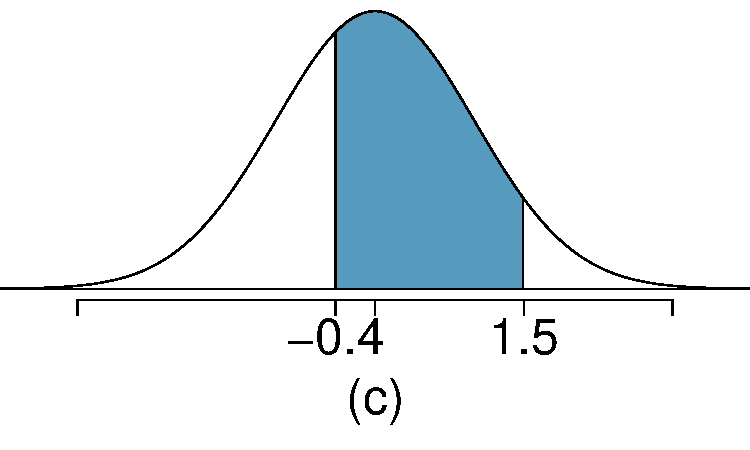
\includegraphics[width=0.2\textwidth]{03/figures/eoce/zBet}
%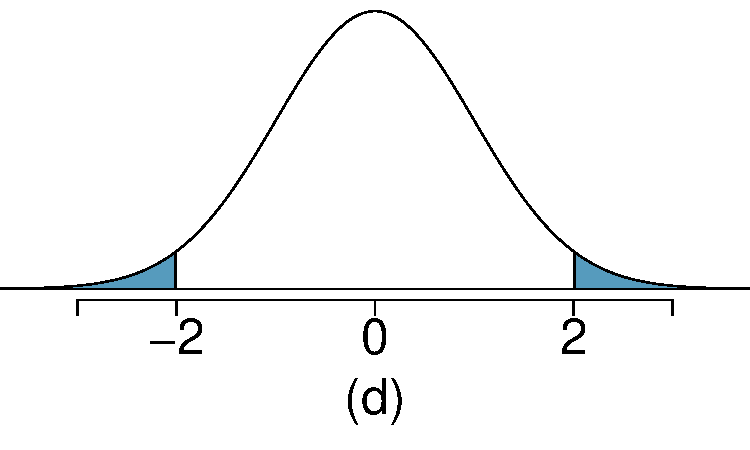
\includegraphics[width=0.2\textwidth]{03/figures/eoce/zgtAbs}

\eoceSol{(a) $X \sim N(\mu = 462, \sigma = 119)$, $Y \sim N(\mu = 584, \sigma = 151)$. (b) $Z_{VR} = 1.33$, $Z_{QR} = 0.57$. Plots below. (c) She scored 1.33 standard deviations above the mean on the Verbal Reasoning section and 0.57 standard deviations above the mean on the Quantitative Reasoning section. (d) Perc$_{VR}=91\%$, Perc$_{QR}=72\%$. (e) Verbal Reasoning. (f) VR: 9\%, QR: 28\%. (g) We cannot compare the raw scores since they are on different scales. Comparing her percentiles is more appropriate for determining how well she did compared to others.}
%\includegraphics[width=50mm]{03/figures/eoce/GRE} \vspace{1mm}

\eoceSol{Answers to (b) and (c) would not change, though we would not draw a Normal curve on which to show these scores. We could not answer parts (d) and (e) since the Z table is only valid for the normal model.}

\eoceSol{(a) 711. (b) 400.}

\eoceSol{Figures below. (a) 0.121. (b) 0.156. (c) 62.68 inches. (d) 43.3\%}
%\includegraphics[width=0.2\textwidth]{03/figures/eoce/heightLt48}
%\includegraphics[width=0.2\textwidth]{03/figures/eoce/heightBet}
%\includegraphics[width=0.2\textwidth]{03/figures/eoce/heightPerc}
%\includegraphics[width=0.2\textwidth]{03/figures/eoce/heightLt54}

\eoceSol{(a) 0.140. (b) 70.6$^o$F or colder.}

\eoceSol{(a) 0.68. (b) $x=\$1800$, $\mu=\$1650$. (c) $\sigma=\$220.58$.}

\eoceSol{\textbf{(a)} The book is 1.8 standard deviations above the mean. Usually we say an observation is unusual when it is 2 or more standard deviations from the mean, so this book is not unusually expensive. \textbf{(b)} 0.233. Figure below. \textbf{(c)} If you are following only one auction and set a maximum bid price that is too low, chances are someone will outbid you and you won't win the auction. If your maximum bid price is too high, you may win the auction but you may be paying more than is necessary. If you are following more than one auction and your maximum bid price is too low, chances are you won't win any of the auctions. However if your maximum bid price is too high, you may win more than one auction and end up with multiples of the same item. \textbf{(d)} A reasonable maximum bid would be the cutoff for the cheapest 10\% of auctions. Even though $10^{th}$ percentile is a reasonable cutoff point, we still may end up being too low and not win any auction. \textbf{(e)} Perhaps a little above the $10^{th}$ percentile: \$69.80.}
%\includegraphics[width=0.2\textwidth]{03/figures/eoce/chemBooks1}\vspace{1mm}

\eoceSol{70\% of the data are within 1 SD, 95\% are within 2 SD, and 100\% are within 3 SD of the mean. The data approximately follow the 68-95-99.7\% Rule.}

\eoceSol{The distribution is unimodal, symmetric, approximately follows the 68-95-99.7\% Rule. The superimposed normal curve approximates the distribution reasonably well. Therefore we can say that the distribution is nearly normal. The points on the Normal probability plot also seem to follow a straight line. However there is one outlier on the lower end that is apparent in both graphs.}

\eoceSol{The points on the Normal probability plot seem to follow a straight line, so we can say that the distribution is nearly normal (or at least we don't have convincing evidence that it is not nearly normal).}
%\includegraphics[width=0.3\textwidth]{03/figures/eoce/QQnorm.pdf}\vspace{1mm}

\eoceSol{No, in poker cards are dealt without replacement.}

\eoceSol{(a) 0.14. (b) 0.0046. (c) $\mu=6$, $\sigma=5.48$.}

\eoceSol{(a) 0.09. (b) $\mu=10$, $\sigma=9.49$.}

\eoceSol{As $p$ gets smaller, i.e. the event is rare, the expected number of trials before a success and the standard deviation increase.}

\eoceSol{(a) 0.096. (b) $\mu=8$, $\sigma= 7.48$.}

\eoceSol{(a) Yes, it meets the four required conditions. (b) 0.291. (c) 0.291.}

\eoceSol{(a) $\mu=34.85$, $\sigma=3.25$. (b) Yes, since 45 is more than 3 standard deviations from the mean. (c) 0.0002.}

\eoceSol{(a) 0.167. (b) 0.997.}

\eoceSol{(a) 0.999. (b) 0.246. (c) 0.246. (d) 0 since the other three tosses must be either heads or tails.}

\eoceSol{(a.i) 0.109. (a.ii) 0.218. (b.i) 0.137. (b.ii) 0.449. (b.iii) 0.551. (b.iv) 0.084.}

\eoceSol{The probability model is below.}
{\scriptsize\begin{tabular}{lllll}
\hline
$Y$	& -3	& -1	& 1	& 3 \\
$P(Y)$	& 0.1458	& 0.3936	& 0.3543	& 0.1063 \\
\hline
\end{tabular}} \vspace{1mm}

\eoceSol{(a) 0.0804. (b) 0.0321. (c) 0.0193.}

\eoceSol{(a) Poisson($\lambda=75$). (b) $\mu=\lambda=75$, $\sigma=\sqrt{\lambda} = 8.66$. (c) $Z=\frac{60 - 75}{8.66} = -1.73$. Since 60 customers is within 2 standard deviations of the mean, this would not be considered unusual.}

\eoceSol{$P(X = 70) = \frac{75^{70} e^{-75}}{70!} = 0.0402$}














\end{document}  